%!TEX root = ../dissertation.tex
\Chapter{Introduction}
% \chapter{Introduction}
\label{introduction}

\newthought{How can we build} theoretically satisfying and practically useful models of the human mind? Historically, there have been two broad approaches. The \emph{rational} approach, exemplified by the work of David Marr (e.g., \citeyear{marr1982vision}) and John Anderson (e.g., \citeyear{anderson1990adaptive}), focuses on characterizing the problems people have to solve and the optimal solutions to those problems. Under the assumption that the mind is well adapted to its environment, these optimal solutions then serve as models of cognition. Rational models are satisfying because they tell us \emph{why} the mind works the way it does, and they are useful because they allow us to make generalizable predictions about how people will behave in new environments (i.e., rationally). However, by construction, such models don't explain \emph{how} the mind achieves the rational ideal, and a growing list of systematic cognitive biases \citep{kahneman2011thinking} draws their predictive utility into question. 

In contrast, the \emph{mechanistic} approach focuses on identifying the cognitive processes underlying behavior, often with an emphasis on explaining the behavioral idiosyncrasies that rational models gloss over. This approach can potentially tell us how the mind actually works, and it can produce extremely accurate models. However, lacking the optimality constraint, there is an enormous space of possible mechanistic models, and they typically have free parameters that are tuned for specific experimental setups. We are thus often left wondering why this specific model fit the data best, and whether it would continue to make good predictions in a slightly different context.

Although the rational and mechanistic approaches have traditionally been viewed as conflicting, the past decade has seen a resurgence of an old idea \citep{simon1955behavioral}: rationality can be seen as a property of cognitive mechanisms themselves. Specificially, a cognitive mechanism is rational if it makes optimal use of limited cognitive resources. Going under various names---cognitively bounded rational analysis \citep{howes2009rational}, computational rationality \citep{lewis2014computational,gershman2015computational}, and resource-rational analysis \citep{griffiths2015rational,lieder2020resourcerational} to name a few---this view suggests that we should not expect people to be rational in the traditional sense of taking actions that maximize expected utility \citep{vonneumann1944theory}. Instead, we should expect people to select actions using mental strategies that strike a good tradeoff between the utility of the chosen action and the cogntive cost of making the decision.

But what defines a ``good'' tradeoff between action utility and cognitive cost? And how can we identify mental strategies that achieve such a tradeoff? In this dissertation, I suggest answers to these questions based on a key insight: \emph{a rational mental strategy is one that optimally solves the sequential decision problem posed by one's internal computational environment}. Under this view, cognition is a problem of stringing together a series of basic cognitive operations, or ``computations'', in the service of choosing what to do in the world. An optimal cogntive process strings those basic operations together in such a way that maximizes the difference between the utility of the ultimate behavior and the total cost of all the cognitive operations that support the behavior.


\section{Sequential decisions in the world and the mind}

\begin{figure}[t]
  \centering
  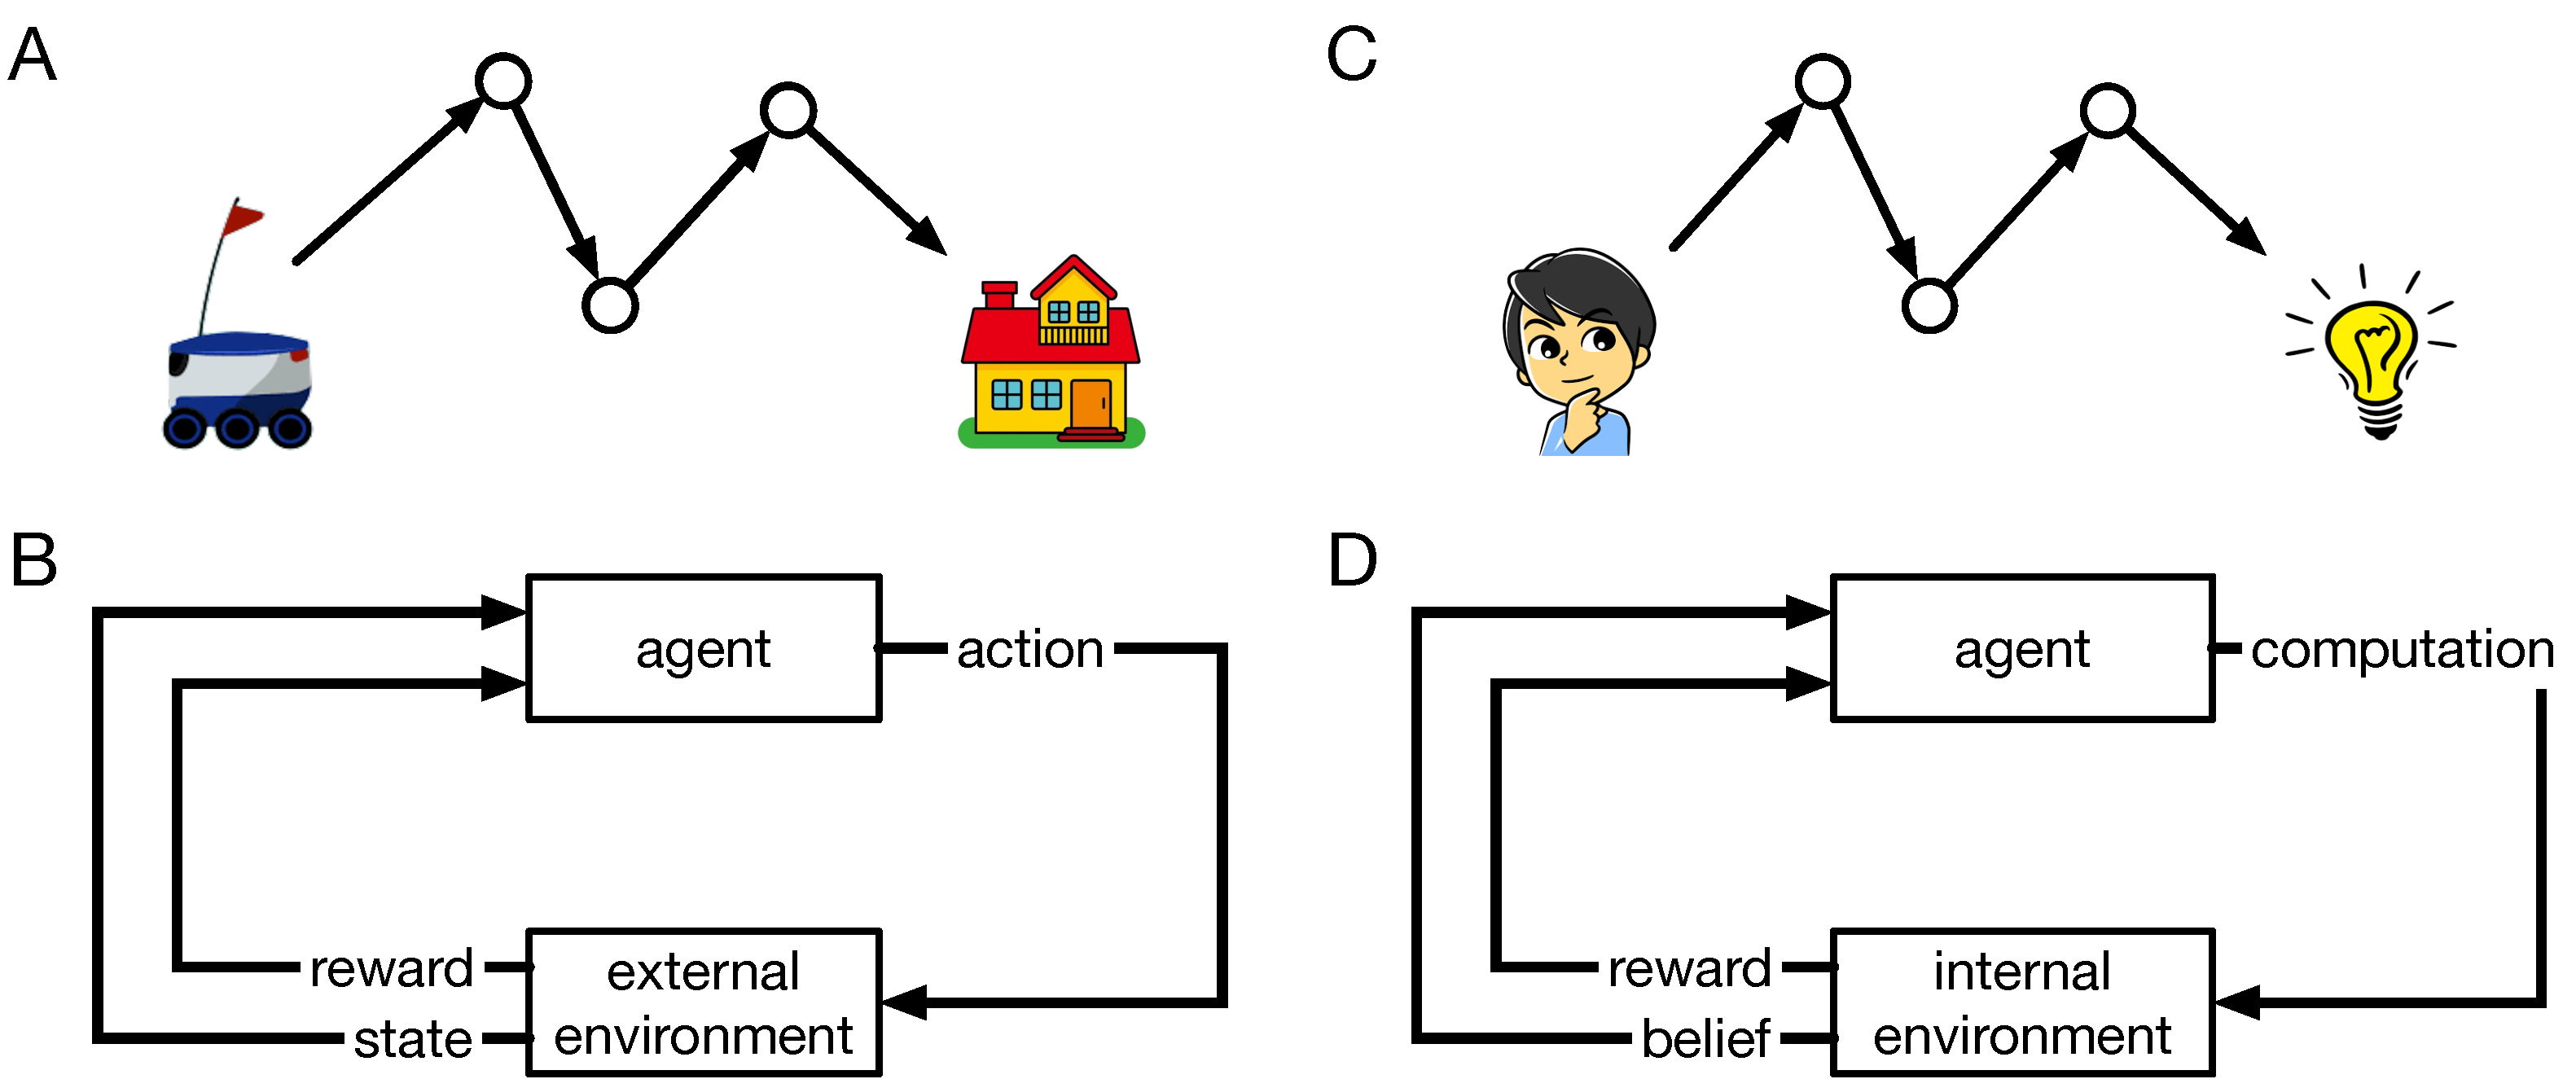
\includegraphics[width=0.9\textwidth]{diagrams/sequential-intuition.pdf}
  \caption{Sequential decision problems posed by external and internal environments.}
  \label{fig:sequential-intuition}
\end{figure}


To make things concrete, consider the problem facing a delivery robot, illustrated in Figure~\ref{fig:sequential-intuition}A. Completing this task will require visiting multiple locations in sequence before arriving at the final destination. And at each location, the robot will need to decide where to go next. Thus, it is a sequential decision problem. Figure~\ref{fig:sequential-intuition}B illustrates how this type of problem is often modeled in artificial intelligence research. At each time step, an agent (here, the robot) takes an \emph{action} (e.g., driving forward). This action causes the environment to enter a new \emph{state} (e.g., one where the robot is in a new location). Additionally, the agent receives a \emph{reward}, a number that captures how good or bad the immediate consequences of the action are. The robot's goal is to maximize the total reward received. For example, the delivery robot might receive a large positive reward for reaching the destination and a small negative reward every time it moves (capturing the desire to conserve battery life). After receving the reward and new state, the agent selects another action and the cycle continues.

Figure~\ref{fig:sequential-intuition}C illustrates a seemingly very different type of situation: a person trying to come up with a solution to a difficult problem. However, as the diagram suggests, the two cases actually share the same basic structure. Both involve an extended interaction between an agent and an environment; but whereas the robot is interacting with an \emph{external} environment, the thinker is interacting with an \emph{internal environment}: their own mind. Just as the robot makes several moves, and visits several locations before reaching the destination, the thinker has several thoughts, and enters several mental states before discovering the solution. Indeed, as illustrated in Figure~\ref{fig:sequential-intuition}D, this problem can be modeled in precisely the same way as the delivery problem. However, now the actions correspond to computations (thoughts) and the states correspond to beliefs (mental states). Thinking changes one's mental state just as moving changes one's physical state; and it also incurs a cost---at the very least, thinking takes time.

An important property of sequential decision problems is that there is often a dissociation between the short-term reward and the long-term \emph{value} of performing some action. For example, if the robot had the option of simply sitting still, this would incur no cost and would thus be the most rewarding action in a myopic sense. However, the potential for the large reward associated with making a delivery makes paying this cost worthwhile. Thus, moving has value. By the same token, a truly myopic agent (one who only considers immediate rewards) would never do any thinking at all! Thinking only has value insofar as it can inform our future behavior.\footnotemark{}

\footnotetext{Note that, subjectively, thought itself can be rewarding (sometimes intensely so; \citealp{gopnik1998explanation}). However, just as with ``secondary reinforcers'' like money, this is not because thought is inherently valuable, but because it is associated with value. Nevertheless, this association may be deeply engrained, perhaps even genetically so. We return to this question in the conclusion.}

The power of identifying this parallel between external and internal environments is that it allows us to leverage existing knowledge about sequential decision problems (a substantial chunk of AI research) to build rational mechanistic models of cognition. That is, we can apply the same formalisms and algorithms that might help a robot deliver groceries to instead characterize the problem of resource-bounded cognition, and identify cognitive processes that optimally solve that problem.


\section{Relation to previous work}



\newcommand{\yes}{\checkmark &}
\begin{table}[tb]
  \caption{Classification of cognitive models.}
  \label{tab:comparison}
  \centering
  \begin{tabular}{ccc|p{\dimexpr\textwidth - 7cm}}
  \toprule
  Dynamic & Bounded & Optimized & Examples \\
  \midrule
  \yes & &
    Evidence accumulation, Cogntive architectures
  \\ & \yes & 
    Heuristics and Biases
  \\ & & \yes
    Rational analysis, Econ
  \\ \yes \yes &
    Ecological rationality
  \\ \yes & \yes 
    ?? Dynamic and optimized ??
  \\ & \yes \yes 
    Expected value of control, Information-theoretic bounded rationality
  \\ \yes \yes \textasciitilde &
    Sampling, 
  \\ \yes \yes \yes
    This dissertation 
  \\ \bottomrule
  \end{tabular}
\end{table}


The proposed approach builds on a long history of cognitive modeling. To understand how this approach is similar to and different from previous approaches, it is useful to highlight its three key assumptions: cognition is \emph{dynamic} (sequential, occuring over time), \emph{bounded} (subject to costs or constraints), and \emph{optimized} (maximizing reward). As illustrated in Table~\ref{tab:comparison}, various combinations of these assumptions are made frequently in models of the mind. However, by capturing all three ideas at once, the current approach has advantages that cannot be achieved with any subset.

The fact that cognitive processes are dynamic is uncontroversial, perhaps even self-evident. Thus, this property is shared by most mechanistic models. One widely used class of dynamic models are \emph{evidence accumulation} (or sequential sampling) models, such as the drift diffusion model \citep{ratcliff1978theory}, the leaky competing accumulator \citep{usher2001time}, and decision by sampling \citep{stewart2006decision}. According to these models, decision making involves accumulating noisy evidence in favor of each possible choice until the evidence for one choice is sufficiently greater than the evidence for the other(s). These models can thus explain not only the choices we make, but also how long it takes to make them.

% A critical property of these models is that they can predict not only what choice people will make, but also how long it will take them to make it. For example, these models predict that easier decisions will be made both more consitently and more quickly, and that mistakes will be faster than correct choices.

% One of the simplest, oldest, and still most widely used dynamic models is the drift diffusion model (DDM) of decision making \tocite. According to this model, making a decision involves accumulating noisy evidence in favor of one decision vs. another until the net evidence exceeds some threshold. A critical property of the DDM and other dynamic models is that it can predict both the choice people will make as well as how long it will take them to make it.

Another important class of dynamic models, \emph{cognitive architectures}, aims to capture a more diverse range of mental activities, beyond simply accumulating more evidence. These models, most notably ACT-R \citep{anderson1996act} and SOAR \citep{laird1987soar}, explicitly model individual cognitive operations such as perceptually encoding a stimulus, recalling information from long-term memory, and performing transformations on symbolic representations of hypothetical world states. 
% These models can trace their intellectual roots to the infancy of artificial intelligence research \citep{newell1956logic}. More ambitious goals... 
However, applying these models in practice poses a substantial challenge. Because any number of cognitive operations could be executed at any time, one must also specify a strategy for how the operations are chosen; in practice this is often done in an ad hoc manner (c.f., \citealp{howes2009rational}).

Optimization, on the other hand, is the defining feature of rational models. Concretely, a cognitive model is optimized if its structure or parameters are set in order to maximize some definition of performance. The prototypical example is expected utility theory \citep{vonneumann1944theory,savage1954foundations}, which simply assumes that people will take actions that maximize their total expected utility. This model is so abstract that it tells us little about cognition itself. However, applying the optimization principle in more constrained domains has yielded important insights about many areas of cognition, including perception \citep{marr1982vision,knill1996perception,najemnik2005optimal} categorization \citep{anderson1991adaptive,ashby1995categorization}, memory \citep{anderson1989human}, and language \citep{goldwater2009bayesian}.


More recently, the notion of optimality has been extended to account not only for the demands imposed by the external environment but also the demands imposed by our own cognitive limitations \citep{howes2009rational,lewis2014computational,gershman2015computational,griffiths2015rational,lieder2020resourcerational}. This approach dates back to Simon \citep{simon1955behavioral} and has been especially useful in the domain of decision-making, where it has been used to explain both how long people deliberate \citep{bogacz2006physics,drugowitsch2012cost,tajima2016optimal,tajima2019optimal,fudenberg2018speed} and also what people think about \citep{callaway2021fixation,jang2021optimal} while making ``simple'' (i.e., non-sequential) choices. However, to the best of our knowledge, there has been no such analysis in the domain of planning, despite the especially critical role that computational limitations play in this case (but c.f. \citep{sezener2019optimizing,mattar2018prioritized} for closely related efforts, which we discuss further below).


The use of optimization in cognitive models is more controversial. 


The basic premise of the approach is that the mind should be well adapted to its environment, through some combination of learning and evolution \citep{anderson1990adaptive}. Optimization simply takes this idea to the logical extreme, assuming that the mind is adapted \emph{as well as possible} to the environment.



% Dynamic: DDMs.

% Control: attention, metacognition.

% Adaptive: rational analysis, economics

% More interesting are models that capture two of the three properties.

% Dynamic + Control: cognitive architectures.

% Dynamic + Adaptive: ???

% Control + Adaptive: EVC


% \newcommand{\yes}{\checkmark &}
% \begin{table}[tb]
%   \caption{Classification of cognitive models.}
%   \label{tab:comparison}
%   \centering
%   \begin{tabular}{cccc|c}\toprule
%   Dynamic & Controlled & Optimized & Notable Examples \\
%   \midrule
%   \yes & &
%     DDM 
%   \\ & \yes &
%     Attention, metacognition 
%   \\ & & \yes
%     Rational analysis, economics 
%   \\ \yes \yes &
%     Cogntive architectures, ecological rationality
%   \\ \yes & \yes 
%     Bogacz ?
%   \\ & \yes \yes 
%     EVC, information-theoretic
%   \\ \yes \yes \yes
%     This dissertation 
%   \\ \bottomrule
%   \end{tabular}
% \end{table}


sampling
information theoretic
rational analysis
ecological rationality
EVC
cognitive architectures

% \begin{table}[tb]
%   \caption{caption here}
%   \label{tab:tablename}
%   \centering
%   \begin{tabular}{ccc|c}\toprule
%   Dynamic & Control & Adaptive & Examples \\
%   \midrule
%   \yes & &     DDM \\
%   & \yes &     Attention, metacognition \\
%   & & \yes     Rational analysis, economics \\
%   \yes \yes &  Cogntive architectures \\
%   \yes & \yes  ? \\
%   & \yes \yes  EVC \\
%   \yes \yes \yes  This dissertation \\
%   \bottomrule
%   \end{tabular}
% \end{table}



In comparison to non-rational dynamic models, the proposed approach
- naturally captures metacognition and control
  - c.f. aDDM which assumes random attention
  - c.f. metamemory which ignores control
- avoids combinatorial search

Compared with non-sequential rational models, 



 % the problem posed by the internal environment (what I will call the \emph{meta-level} problem) is exactly analagous to the problem posed by the external environment (the \emph{object-level} problem). 








In comparison to non-dynamic rational models
- captures the process/mechanism (c.f. information-theoretic accounts)
- more optimal
- captures sequential dependence



% Taken from planning (cut there?)
These challenges---hypothesis generation, generalizable prediction, and functional explanation---are not unique to planning; indeed, they arise in nearly all areas of cognition. In many domains, progress in addressing these challenges has been made by analyzing optimal solutions to the problem a cognitive system is meant to solve \citep{marr1982vision,anderson1990adaptive}. This approach has generated insight into a wide range of problems, including decision-making \citep{savage1954foundations}, generalization \citep{tenenbaum2001generalization}, categorization \citep{anderson1991adaptive,ashby1995categorization}, perception \citep{knill1996perception}, and information-seeking \citep{oaksford1994rational,gureckis2012selfdirected}. More recently, the notion of optimality has been extended to account not only for the demands imposed by the external environment but also the demands imposed by our own cognitive limitations \citep{howes2009rational,lewis2014computational,gershman2015computational,griffiths2015rational,lieder2020resourcerational}. This approach dates back to Simon \citep{simon1955behavioral} and has been especially useful in the domain of decision-making, where it has been used to explain both how long people deliberate \citep{bogacz2006physics,drugowitsch2012cost,tajima2016optimal,tajima2019optimal,fudenberg2018speed} and also what people think about \citep{callaway2021fixation,jang2021optimal} while making ``simple'' (i.e., non-sequential) choices. However, to the best of our knowledge, there has been no such analysis in the domain of planning, despite the especially critical role that computational limitations play in this case (but c.f. \citep{sezener2019optimizing,mattar2018prioritized} for closely related efforts, which we discuss further below).



\section{Optimal cognitive processes as solutions to Markov decision processes}

The proposed approach rests on a key intuition: the thoughts one has at any moment depend on the thoughts one had before. That is, our mental processes are sequentially dependent. Furthermore, thoughts are only useful insofar as they influence our behavior, and this behavior often occurs well after the thought itself. That is, the benefits of thought are temporally delayed. These two properties, sequential dependence and delayed reward make sequential decision problems very challenging to solve. Fortunately, a long history of work in artificial intelligence---from Newell and Simon's pioneering proof-writing programs \citep{newell1956logic} to super-human Chess and Go engines \citep{silver2017mastering}---has focused on solving just this sort of problem.

In artificial intelligence research, sequential decision problems are often formalized with the framework of \textbf{Markov decision processes (MDP)} \citep{puterman2014markov,sutton2018reinforcement}. An MDP describes a dynamic interaction between an agent and an environment. It is defined by a set of possible states the environment can be in, a set of actions the agent can execute, a reward function that specifies the immediate utility associated with executing each action in each state, and a transition function that specifies how actions change the state. The agent's goal is to maximize the total cumulative reward received. This can be accomplished by choosing actions according to the optimal policy, which specifies the best action to execute in each state. See Box~1 for a technical definition of MDPs.

% In addition to their foundational role in artificial intelligence \citep{sutton2018reinforcement}, MDPs are widely used in models of human decision-making \citep{dayan2008decision}. MDPs are the formal foundation for models of reinforcement learning \citep{niv2009reinforcement} and model-based planning \citep{huys2015interplay,botvinick2012planning}, as well as competition between the two systems \citep{daw2005uncertaintybased,keramati2011speed,kool2017costbenefit}. They have also been used to study information-seeking \citep{gottlieb2013informationseeking,hunt2016approachinduced}, generalization \citep{tomov2021multitask}, and hierarchical abstraction \citep{solway2014optimal,botvinick2009hierarchically}. However, with a few notable exceptions \citep{dayan2008serotonin,drugowitsch2012cost,tajima2016optimal}, MDPs have primarily been used to model the sequential decision problems posed by the external world. In the following section, we show how this framework can be applied to model the sequential decision problem posed by one's own cognitive architecture.

The fact that cognition---or more generally, computation---poses a sequential decision problem was recognized by researchers in the field of \textbf{rational metareasoning}, which aims to build AI systems that can adaptively allocate their limited computational resources. In particular, Hay and colleagues \citealp{hay2012selecting,hay2016principles} formalize this problem of ``selecting computations'' as a \textbf{metalevel MDP}. In a metalevel MDP, the states correspond to beliefs and the actions correspond to computations that refine those beliefs (according to the transition function). The reward function encodes both the costs and benefits of computation; it assigns a strictly negative reward for each computation executed, but a potentially positive reward for the utility of the external action that is ultimately chosen (based on the belief produced by computation).

Applying the metalevel MDP formalism to cognitive science provides a suite of theoretical and computational tools, both to formalize the problems that our brains must solve, and to identify near-optimal solutions to those problems. In a psychological context, the states of a metalevel MDP can be interpreted as mental states, and the actions as cognitive operations. Along with the transition function, these specify the environment ``within the skin'' that a cognitive process must interact with. By further specifying a reward function, we can quantify the tradeoff between cognitive cost and extrinsic utility . This in turn allows us to identify the optimal cognitive process---that is, the one achieves the best possible tradeoff between cost and utility---as the optimal policy for the metalevel MDP.